\documentclass[11pt]{article}
\usepackage[utf8]{inputenc}
\usepackage[top=60pt, bottom=60pt, left=70pt, right=70pt]{geometry}
\usepackage{graphicx,amsmath}
% Default fixed font does not support bold face
\DeclareFixedFont{\ttb}{T1}{txtt}{bx}{n}{8} % for bold
\DeclareFixedFont{\ttm}{T1}{txtt}{m}{n}{8}  % for normal
% Custom colors
\usepackage{color}
\definecolor{deepblue}{rgb}{0,0,0.5}
\definecolor{deepred}{rgb}{0.6,0,0}
\definecolor{deepgreen}{rgb}{0,0.5,0}
\definecolor{commentgrey}{rgb}{0.5,0.5,0.5}
\usepackage{listings}

% Python style for highlighting
\lstset{
language=Python,
basicstyle=\ttm,
otherkeywords={self},             % Add keywords here
keywordstyle=\ttb\color{deepblue},
emph={MyClass,__init__},          % Custom highlighting
emphstyle=\ttb\color{deepred},    % Custom highlighting style
stringstyle=\color{deepgreen},
frame=tb,                         % Any extra options here
commentstyle=\color{commentsgrey}
}


\title{Drips Model}
\author{Daniel W. Zaide}

\begin{document}
\maketitle
This document describes the drips model in Drips.py, src/drips.py, and src/drips\_support.py. It is a simple two component model, stacked together similar to ICSolar.\\
\noindent In (1)\\\\
\begin{tabular}{l|l}
Air Energy & $\dot{m}_1(h_1-h_0) = h_e (T_e-T_1) + h_r(T_r-T_1)$ \\
Air Mass & $\dot{m}_1 = \dot{m}_0$ \\
Vapor Mass & $\dot{m}^v_1 = \dot{m}^v_0$
\end{tabular}\\\\
In (2)\\\\
\begin{tabular}{l|l}
Water Energy & $\dot{m}_2^w T_2^w =  \dot{m}_2^wT_2$\\
Water Mass & $m_2^w = m_2^w(0) + \displaystyle \int_0^t \dot{m}_2^w(t')\mathrm{d}t'$ \\
Air Energy & $\dot{m}_{2}h_{2} = \dot{m}_{1}h_{1} - \dot{m}_{2}^w(C_{p}^vT_{2}-\dot{m}_2^wh^e)$\\
Air Mass & $\dot{m}_2 = \dot{m}_1 - \dot{m}_2^w$ \\
Vapor Mass & $\dot{m}_2^v = \dot{m}_1^v - \dot{m}_2^w$
\end{tabular} \\\\

where $v$ is the vapor, and $w$ is the water region respectively. Further, we have $h_{i}$, the enthalpy of air and vapor defined as
\begin{equation}
h_{i} = (1-\chi_i)C_{p,a}T_{i} + \chi_i(h_v+C_{p,v}T_{i})
\end{equation}
with the vapor mass fraction, $\chi_i = \dot{m}^v_i/\dot{m}_i$, and $h^e$, the enthalpy of vaporization. We also have $\dot{m}_i^w = q(\chi_i,m_i^w)$. We can approximate the water mass in time with 
\[
m_i^w(t+\Delta t) = \displaystyle\int_t^{t+\Delta t} \dot{m}_i^w(t')\mathrm{d}t' \approx m_i^w(t) + \Delta t \dot{m}^w_i(t)
\]

Further, defining $\phi$ as the relative humidity $(\phi \in [0,1])$, we can define the weight fraction in kg/kg of vapor to air as
\[
W = \frac{0.62198 \phi P_{vsat}(T)}{(p-\phi P_{vsat}(T))}
\]
where the saturation vapor pressure can be computed from the Antoine equation
\[
\log_{10}P_{vsat}(T) = \left(8.07131-\frac{1730.63}{233.426+T}\right)133.322368
\]
with $T$ in degrees Celcius. At 25 $^{\circ}$C, this is around 0.02 kg water per kg air. We can also compute the air density from relative humidity, air pressure, and temperature as 
\[
\rho = \frac{p}{286.9(273.15+T)}\frac{1+W}{1+1.609W}
\]

To model the rate of water adsorption, we assume an exponential decay as the desiccant saturates, that is
\[
q^w = (m^w_{sat}-m^w)\frac{\ln(2)}{\tau_{1/2}}
\]
where $m^w_{sat}$ is the total amount of mass (in kg) and $\tau_{1/2}$ is the half-life, the time it takes for the desiccant to reach half saturation. If $m^w_{sat} = m^w_{sat}(\phi,T,\ldots)$ then exact exponential decay will not be observed, but the overall behavior will be similar.
\newpage
\begin{figure}[!ht]
\centering
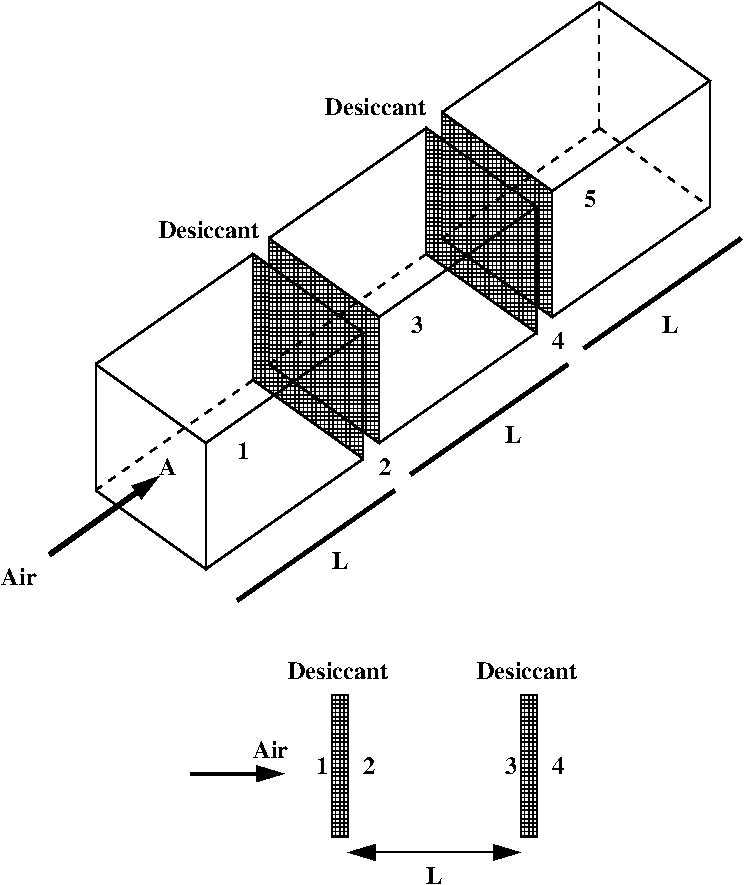
\includegraphics[width=0.8\textwidth]{images/drips.png}
\end{figure}


\end{document}
